\documentclass[11pt]{article}

% Change "review" to "final" to generate the final (sometimes called camera-ready) version.
% Change to "preprint" to generate a non-anonymous version with page numbers.
% arXiv preprint: non-anonymous, no line numbers, no page-limit enforcement.
\usepackage[preprint]{acl}

% Standard package includes
\usepackage{times}
\usepackage{latexsym}
\usepackage{algorithm}
\usepackage{algorithmic}

% For proper rendering and hyphenation of words containing Latin characters (including in bib files)
\usepackage[T1]{fontenc}
\usepackage[utf8]{inputenc}

% This is not strictly necessary, and may be commented out,
% but it will improve the layout of the manuscript,
% and will typically save some space.
\usepackage{microtype}

% This is also not strictly necessary, and may be commented out.
% However, it will improve the aesthetics of text in
% the typewriter font.
\usepackage{inconsolata}

% Including images in your LaTeX document requires adding additional package(s)
\usepackage{graphicx}
\usepackage{booktabs}
\usepackage{amsmath}
\usepackage{amssymb}
\usepackage{multirow}
\usepackage{subcaption}
\usepackage{url}

\title{AdaMem: Learning What to Remember for Personalized Long-Horizon LLM Agents}

% Author information can be set in various styles:
% For several authors from the same institution:
% \author{Author 1 \and ... \and Author n \\
%         Address line \\ ... \\ Address line}
% if the names do not fit well on one line use
%         Author 1 \\ {\bf Author 2} \\ ... \\ {\bf Author n} \\
% For authors from different institutions:
% \author{Author 1 \\ Address line \\  ... \\ Address line
%         \And  ... \And
%         Author n \\ Address line \\ ... \\ Address line}
% To start a separate ``row'' of authors use \AND, as in
% \author{Author 1 \\ Address line \\  ... \\ Address line
%         \AND
%         Author 2 \\ Address line \\ ... \\ Address line \And
%         Author 3 \\ Address line \\ ... \\ Address line}

\author{%
  Xingyu Chen \\
  Shanghai Jiao Tong University, Tencent \\
  \texttt{galaxychen@sjtu.edu.cn}
  \And
  Rui Wang\thanks{\ \ Corresponding authors.} \\
  Shanghai Jiao Tong University \\
  \texttt{wangrui12@sjtu.edu.cn}
  \AND
  Zhaopeng Tu\footnotemark[\value{footnote}] \\
  Tencent \\
  \texttt{tuzhaopeng@gmail.com}
  \And
  Liefeng Bo \\
  Tencent \\
  \texttt{liefengbo@gmail.com}}

\begin{document}
\maketitle
\begin{abstract}
Long-term memory systems for Large Language Model (LLM) agents typically try to \emph{remember everything}, extracting memories uniformly to retain as many facts as possible. In production, however, inference cost and finite context budgets make this untenable: beyond consolidating raw dialogue into memory, an agent must exert \emph{write control}, efficiently keeping only the information each user actually cares about. Otherwise, long-horizon personalized interactions suffer \emph{memory bloat}, where irrelevant trivia crowds out useful information and steadily erodes question-answering (QA) accuracy. We argue that what is worth remembering is role-dependent, and propose \textbf{AdaMem} (Adaptive Memory), a method that \emph{learns what to remember} for each user from feedback. AdaMem maintains a structured, role-specific Memory Policy and refines it from weekly QA feedback through a lightweight, patch-style self-reflection step with failure rollback. To study this setting, we build \textbf{AdaMem-Bench}, a benchmark that simulates weeks of interaction with week-by-week QA. Across two extraction models and two feedback modes, AdaMem improves QA accuracy by up to \textbf{+9.0\%} over the uniform Mem0 baseline while shrinking memory volume by \textbf{9\%}.
\end{abstract}

\section{Introduction}
Large Language Model (LLM) agents are increasingly deployed in long-horizon personalized scenarios, where consistent long-term memory underpins trust and personalization \cite{park2023generative, wang2023survey}. To overcome context-window limits, existing memory systems (e.g., Mem0, MemoryBank) adopt a Retrieval-Augmented Generation (RAG) architecture \cite{lewis2020retrieval, packer2023memgpt, zhong2023memory} and operate under a \textit{uniform extraction rule}: they try to remember everything, saving every factual statement on the assumption that more is better. In real-world deployment, this collides with two hard constraints---inference cost and a finite context budget---since every memory that is later retrieved consumes tokens and latency. Consolidating raw dialogue into memory is therefore not enough: an agent must also \emph{control what it writes}, retaining only the information each user cares about.

As interactions span weeks or months, this uniformity backfires, producing \textbf{memory bloat}: the memory bank accumulates irrelevant trivia (e.g., casual greetings, minor scheduling details) that crowds out the memories that matter at retrieval time, steadily degrading QA accuracy (Figure \ref{fig:motivating}).

\begin{figure}[t]
    \centering
    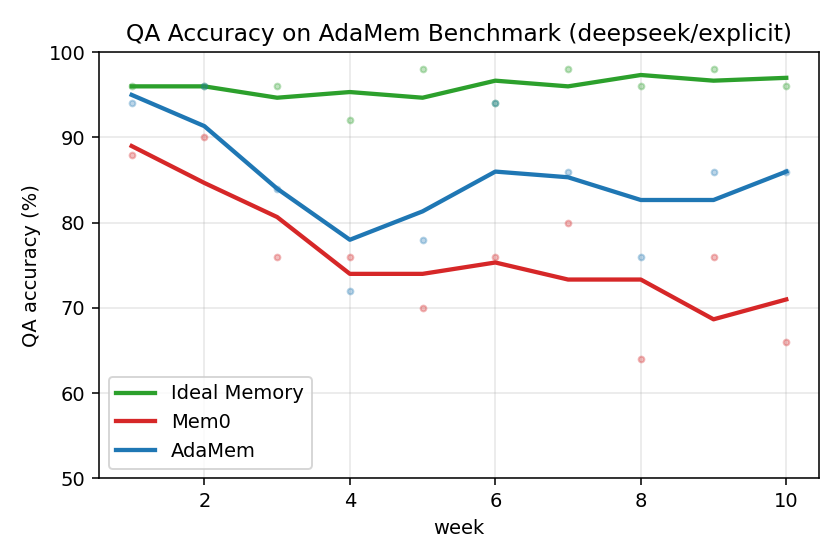
\includegraphics[width=\columnwidth]{f1_motivating_deepseek_verbose.png}
    \caption{Motivating results on AdaMem-Bench (DeepSeek-V4-Flash, Explicit feedback). Accuracy over 10 weeks (smoothed with window $w=3$). Ideal Memory and AdaMem maintain high performance, while the uniform Mem0 baseline degrades over time.}
    \label{fig:motivating}
\end{figure}

Our key insight is that an agent should not remember everything, but instead \textbf{learn what to remember}, because what counts as important is subjective and role-dependent: an agent talking to a manager should track business decisions, whereas one chatting with a fitness buddy should track workout schedules. Memory extraction should therefore be guided by a \textit{Memory Policy} aligned with each user's preferences and continually corrected from feedback.

We realize this idea in \textbf{AdaMem}, a preference-guided extraction framework that runs a closed-loop weekly cycle: (1) \textbf{Daily Extraction} stores memories under a structured Memory Policy; (2) \textbf{Weekly Evaluation} probes the agent via QA; (3) \textbf{Policy Reflection} diagnoses the resulting errors and emits a ``patch'' that updates the policy, guarded by a failure-rollback check; and (4) \textbf{Policy Rendering} compiles the policy into the next week's extraction instructions, including a \textbf{Time Anchoring} step that resolves relative dates.

\paragraph{Contributions} (1) We reframe long-horizon memory for industrial deployment as a \emph{write-control} problem: under real-world inference-cost and context budgets, an agent should keep only user-relevant information rather than consolidate dialogue wholesale, turning extraction into an actively managed, preference-aligned process. (2) We propose \textbf{AdaMem}, which learns a role-specific Memory Policy from feedback and applies patch-style reflection with failure rollback to decide what to write---a lightweight recipe that drops into existing RAG memory stacks. (3) We build \textbf{AdaMem-Bench}, a personalized long-horizon benchmark with golden-memory annotations, and show that across two extraction LLMs and two feedback modes AdaMem improves QA accuracy by up to \textbf{+9.0\%} while shrinking memory volume by \textbf{9\%}; our analysis localizes the gains to ``soft preference'' categories (emotions, promises, schedules) and identifies policy inference from weak feedback as the primary remaining bottleneck.\footnote{Our code, the AdaMem-Bench benchmark, and reproduction artifacts are available at \url{https://github.com/galaxyChen/AdaMem}.}

\section{Related Work}
\paragraph{Long-Term Memory and Hierarchical Storage}
Long-term memory is essential for LLM agents in long-horizon interactions \cite{wang2023survey}. Early works retrieve raw chat history \cite{park2023generative} or extract atomic facts \cite{mem0, zhong2023memory}. To handle context limitations, MemGPT \cite{packer2023memgpt} and MemoryOS \cite{memoryos2025} use hierarchical storage paging. Graph-based architectures like MemInsight \cite{meminsight2025} and All-Mem \cite{allmem2026} build topological relations to prevent structure drift, while systems like Temporal Semantic Memory (TSM) \cite{tsm2026} organize events along semantic timelines to resolve temporal reasoning.

\paragraph{Personalization, Preference Alignment, and Alleviating Bloat}
To personalize agent behavior \cite{modarressi2023retrieval}, systems like PersonaAgent \cite{personaagent2025}, PersonaMem \cite{personamem2025}, and Dynamic Affective Memory \cite{affectivemem2025} align agent actions or emotions using retrieved long-term memory. Yet they still remember everything at extraction time, so the underlying store suffers from memory bloat. SimpleMem \cite{simplemem2026} applies semantic compression and Nemori \cite{nemori2025} uses predictive-coding theory to trigger storage on prediction gaps, but both compress \emph{after} the fact. AdaMem instead decides \emph{what to remember} upfront, via a structured, role-specific Memory Policy that guides extraction.

\paragraph{Active Memory Policies and Self-Reflective Loops}
Memory management has shifted from static heuristics to active policies. AgeMem \cite{agemem2026}, for instance, frames CRUD operations as an action space trained via GRPO. For self-correction, dialogue systems adopt reflective memory management (RMM) \cite{prospectretro2025} for prospection and retrospection, while EvolveMem \cite{evolvemem2026} learns retrieval configurations from failure logs. Unlike task- or code-level reflection \cite{shinn2023reflexion, madaan2023self}, AdaMem applies patch-style reflection to the \emph{extraction policy} itself, iteratively refining the natural-language rules that decide what to remember for each role---and, in doing so, exposes policy inference as the key bottleneck.

\section{Method: AdaMem}
AdaMem learns what to remember for each user by aligning memory extraction with their preferences through a closed-loop weekly cycle (Algorithm \ref{alg:adamem_pipeline}): daily extraction, weekly evaluation, feedback diagnostics, adaptive policy updates, and final QA writeback.

\begin{algorithm}[t]
\caption{AdaMem Pipeline}
\label{alg:adamem_pipeline}
\begin{algorithmic}[1]
\REQUIRE Dialogue history $\{S_{t,d}\}$, initial Policy $\mathcal{P}_1$, Database $\mathcal{D} \leftarrow \emptyset$.
\FOR{week $t = 1, \dots, T$}
    \FOR{each day $d$ of week $t$}
        \STATE Resolve relative temporal references in $S_{t,d}$
        \STATE Extract preference memories $\mathcal{M}_{t,d}$ guided by policy $\mathcal{P}_t$
        \STATE $\mathcal{D} \leftarrow \mathcal{D} \cup \mathcal{M}_{t,d}$
    \ENDFOR
    \STATE Answer weekly QA $\mathcal{Q}_t$ using retrieved context from $\mathcal{D}$
    \STATE Receive feedback; identify incorrect answers $\mathcal{W}_t$
    \IF{$\mathcal{W}_t \neq \emptyset$}
        \STATE Reflect on failures to diagnose recall/precision errors
        \STATE Propose policy patch $\Delta \mathcal{P}_t$: $\mathcal{P}_{t+1}' \leftarrow \mathcal{P}_t \oplus \Delta \mathcal{P}_t$
        \STATE If historical validation improves, update $\mathcal{P}_{t+1} \leftarrow \mathcal{P}_{t+1}'$, else rollback $\mathcal{P}_{t+1} \leftarrow \mathcal{P}_t$
    \ELSE
        \STATE Maintain policy: $\mathcal{P}_{t+1} \leftarrow \mathcal{P}_t$
    \ENDIF
    \STATE Regenerate answers with updated memory and write back
\ENDFOR
\end{algorithmic}
\end{algorithm}

\subsection{Memory Policy Structure}
The \textbf{Memory Policy} $\mathcal{P} = \{ C_1: \mathcal{T}_1, \dots, C_n: \mathcal{T}_n \}$ is a JSON object mapping characters $C_i$ to their natural language extraction preferences $\mathcal{T}_i$ (e.g., ``Only extract final business decisions and deadlines; ignore daily chit-chat'').

\subsection{Patch-Style Reflection and Update}
At the end of each week, the agent reflects on incorrect QA pairs $\mathcal{W}_t$ and diagnoses failures as: (1) \textbf{Recall Failure (Missing Memory)} where the dialogue had the info but the extractor missed it (policy too restrictive); or (2) \textbf{Precision Failure (Noisy Memory)} where irrelevant retrieved memories misled the answering model (policy too permissive).

Based on this, the agent generates a \textbf{policy patch} $\Delta \mathcal{P}_t$ to adjust $\mathcal{T}_i$. To ensure stability and prevent policy drift, AdaMem employs a \textbf{failure rollback} mechanism: if the updated policy degrades validation performance on historical QA pairs, the update is rejected and the policy rolls back.

\subsection{Rendering and Time Anchoring}
During daily extraction, the active policy $\mathcal{P}$ is rendered as custom instructions (e.g., ``\textit{Extract memories strictly according to the following character preferences...}'') in the extractor's prompt.

\paragraph{Time Anchoring}
Relative temporal references (e.g., ``tomorrow'') become misleading if saved verbatim. AdaMem injects the session's absolute date into the extraction prompt and instructs the LLM to resolve all relative expressions into absolute dates before saving (e.g., ``Meeting scheduled for June 18, 2026'').

\section{AdaMem-Bench and Setup}
We construct \textbf{AdaMem-Bench}, a personalized long-horizon benchmark with session-level golden-memory annotations, to evaluate the AdaMem method.

\subsection{Dataset and Data Synthesis}
To evaluate preference-guided memory systems under realistic settings, we build AdaMem-Bench around three design principles:
\begin{itemize}
    \item \textbf{Realistic conversational dynamics.} We simulate natural, multi-session dialogues that embed casual chit-chat, temporal references, and subjective nuances, rather than single-turn or template-based text.
    \item \textbf{Multi-persona memory tracking.} Each environment involves concurrent interactions with several characters, each with distinct roles and information preferences, so the agent must track persona-specific memory and retrieve accordingly.
    \item \textbf{Homogeneous concept interference.} Dialogues are designed with high semantic overlap across characters (e.g., several people discussing fitness schedules), and these same-category distractors stress whether the system confuses similar but irrelevant content from other personas.
\end{itemize}

Our data synthesis pipeline consists of four main stages:
\paragraph{Scenario and Persona Initialization} We initialize $N$ long-term interactive stories, each involving an assistant interacting with $C$ characters. Each character is assigned a distinct preference profile (e.g., schedules, emotional states, deadlines) representing their ground-truth preferences.
\paragraph{Multi-Session Dialogue Generation} We simulate daily dialogues across $T$ weeks using a multi-agent pipeline, naturally embedding key events, factual information, and casual chit-chat.
\paragraph{Golden Memory Annotation} Each dialogue is annotated with session-level ``golden memories'' (atomic facts matching characters' preferences), treating other details as noise.
\paragraph{Preference-Aligned QA Generation} At each week's end, we generate QA pairs targeting only preference-aligned information to test the agent's long-term recall.

\begin{table*}[t]
\centering
\small
\begin{tabular}{lcccc}
\toprule
\textbf{Benchmark} & \textbf{Memory Typology} & \textbf{Pref.-Aware?} & \textbf{Feedback?} & \textbf{Evaluation} \\
\midrule
MemoryBank \cite{zhong2023memory} & Factual QA & No & No & Static Retrieval \\
LoCoMo \cite{maharana2024lococmo} & Event, Factual & No & No & Static QA/Summ. \\
LongMemEval \cite{wu2024longmemeval} & Multi-session Reasoning & No & No & Static Capabilities \\
EverMemBench \cite{evermembench2026} & Persona, Factual & Partial & No & Fine-grained Recall \\
\midrule
\textbf{AdaMem-Bench (Ours)} & \textbf{Personalized Soft Prefs} & \textbf{Yes} & \textbf{Yes} & \textbf{Dynamic Closed-Loop} \\
\bottomrule
\end{tabular}
\caption{Comparison of AdaMem-Bench with existing long-term memory datasets and benchmarks.}
\label{tab:benchmark_comparison}
\end{table*}

\subsection{Baselines and Temporal Alignment}
We compare AdaMem against three baseline methods processed in the same chronological order:
(1) \textbf{Full Context}: A theoretical upper bound where the entire raw history is fed directly into the LLM context.
(2) \textbf{Ideal Memory}: A bound where only human-annotated ``golden memories'' are stored.
(3) \textbf{Mem0}: A widely used uniform extraction baseline \cite{mem0} that remembers everything, extracting all factual information without preference guidance.

QA answers are always produced by \texttt{deepseek-v4-flash}; the two models we vary (DeepSeek-V4-Flash and Gemini-3.5-Flash) are the \emph{extraction} models used by Mem0 and AdaMem. Because Full Context and Ideal Memory involve no memory extraction or policy update, they are extractor-independent and reported once rather than per model.

\subsection{Feedback Modes}
We evaluate two feedback modes after incorrect QA answers:
(1) \textbf{Explicit Feedback}: The user provides the correct answer and explains their preference (e.g., ``\textit{Incorrect. You should remember this because I only care about schedules}'').
(2) \textbf{Implicit Feedback}: The user only provides the correct answer, and the agent must implicitly infer the underlying preference.

\subsection{Evaluation Metrics}
We employ a decoupled evaluation methodology:
\paragraph{QA Accuracy} The percentage of weekly QA questions answered correctly, evaluated by a decoupled \texttt{deepseek-v4-flash} judge.
\paragraph{Extraction F1} The harmonic mean of Precision (the proportion of extracted memories matching user preferences) and Recall (the proportion of successfully extracted golden memories). Note that precision here is preference-based, not factual.
\paragraph{Memory Efficiency Ratio (MER)} Measures the trade-off between QA accuracy and memory volume, defined as:
\begin{equation}
\mathrm{MER} = \frac{\mathrm{Acc} / \mathrm{MemVol}}{\mathrm{Acc}_{\mathrm{Ideal}} / \mathrm{MemVol}_{\mathrm{Ideal}}}
\end{equation}
normalized against Ideal Memory ($\mathrm{MER}_{\mathrm{Ideal}} = 1.0$), showing how efficiently each memory contributes to accuracy.

\begin{figure*}[t]
    \centering
    \begin{subfigure}[b]{0.63\textwidth}
        \centering
        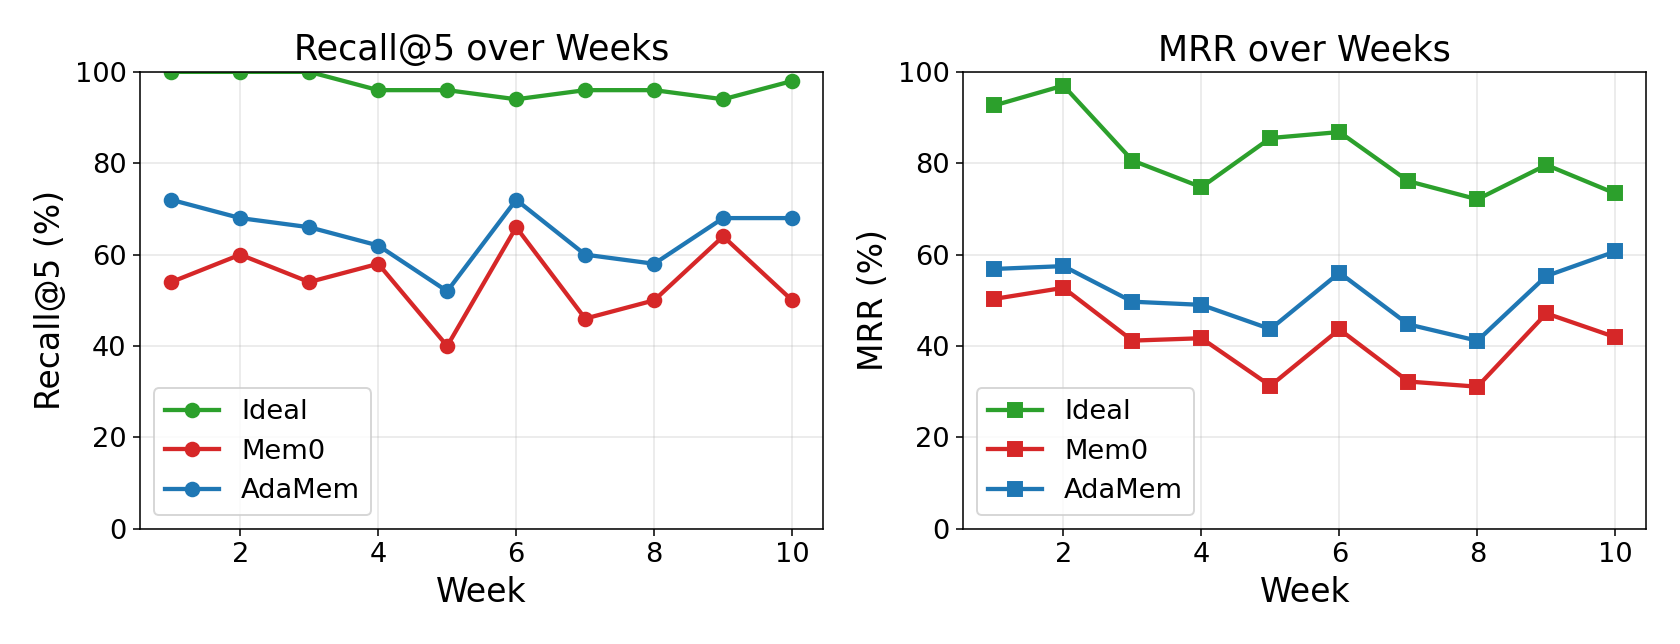
\includegraphics[width=\linewidth]{a9_recall_rank_drift_deepseek_verbose.png}
        \caption{Retrieval quality (Recall@5 and MRR) over 10 weeks.}
        \label{fig:recall_drift}
    \end{subfigure}
    \hfill
    \begin{subfigure}[b]{0.35\textwidth}
        \centering
        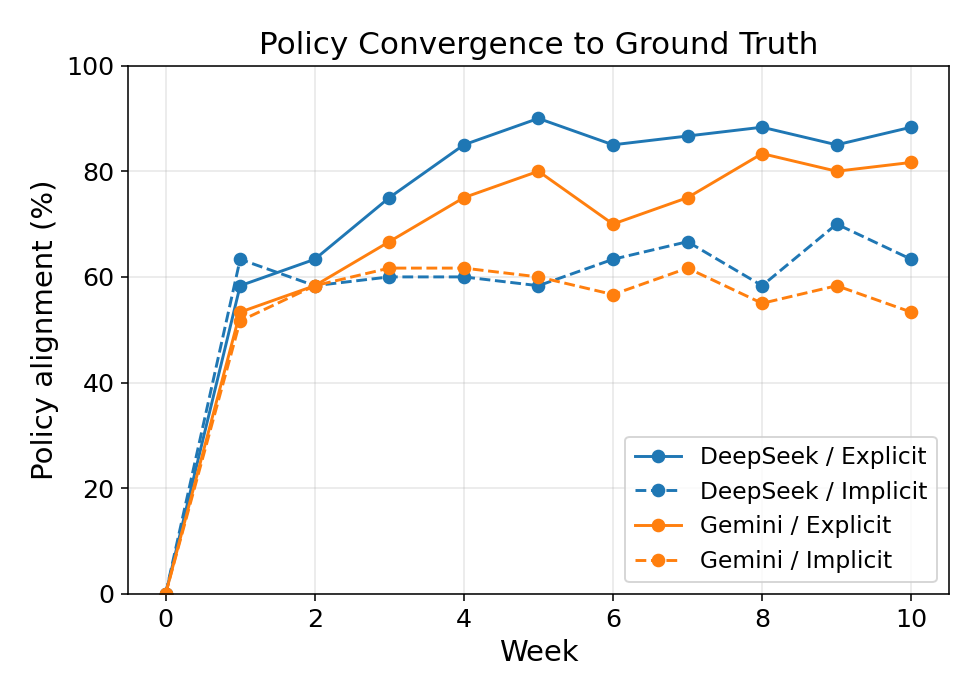
\includegraphics[width=\linewidth]{a4_policy_convergence.png}
        \caption{Policy convergence over 10 weeks.}
        \label{fig:convergence}
    \end{subfigure}
    \caption{Analysis of retrieval dynamics and policy convergence over a 10-week horizon. (a) Recall@5 (left) and Mean Reciprocal Rank (MRR, right) for DeepSeek-V4-Flash under explicit feedback. (b) Semantic alignment of the learned policies with ground-truth preferences.}
    \label{fig:dynamics_and_convergence}
\end{figure*}

\section{Results and Analysis}
We evaluate AdaMem to answer four research questions:
\begin{itemize}
    \item \textbf{RQ1 (Overall Performance)}: Does AdaMem outperform the uniform memory baseline in terms of QA accuracy and memory compactness across different models and feedback modes?
    \item \textbf{RQ2 (Information Categories)}: Where do the performance gains of AdaMem come from when analyzed across different categories of user preferences?
    \item \textbf{RQ3 (Retrieval Dynamics)}: How does AdaMem affect retrieval quality and mitigate memory bloat over extended multi-week interaction horizons?
    \item \textbf{RQ4 (Policy Learning)}: What is the primary bottleneck in preference-guided memory: policy adherence (following instructions) or policy inference (learning preferences from feedback)?
\end{itemize}

\subsection{RQ1: Overall Performance and Memory Efficiency}
Table \ref{tab:main_results} presents results across all methods, models, and feedback modes.

\begin{table*}[t]
\centering
\small
\begin{tabular}{lcccccccc}
\toprule
\multirow{3}{*}{\textbf{Method}} & \multicolumn{8}{c}{\textbf{Feedback Mode}} \\
\cmidrule(lr){2-9}
& \multicolumn{4}{c}{\textbf{Explicit}} & \multicolumn{4}{c}{\textbf{Implicit}} \\
\cmidrule(lr){2-5} \cmidrule(lr){6-9}
& \textbf{Acc (\%)} & \textbf{F1 (\%)} & \textbf{MER} & \textbf{Vol.} & \textbf{Acc (\%)} & \textbf{F1 (\%)} & \textbf{MER} & \textbf{Vol.} \\
\midrule
\multicolumn{9}{l}{\textit{Reference bounds (extractor-independent; QA by \texttt{deepseek-v4-flash})}} \\
Full Context & 96.4 & --- & --- & 0 & 97.2 & --- & --- & 0 \\
Ideal Memory & 96.0 & 97.9 & 1.000 & 121 & 96.4 & 99.4 & 1.000 & 110 \\
\midrule
\multicolumn{9}{l}{\textit{Extraction model: DeepSeek-V4-Flash}} \\
Mem0 & 76.2 & 35.0 & 0.223 & 430 & 80.2 & 33.9 & 0.225 & 407 \\
\textbf{AdaMem} & \textbf{85.2} \scriptsize{(+9.0)} & \textbf{40.1} & \textbf{0.289} & \textbf{371} & \textbf{82.0} \scriptsize{(+1.8)} & \textbf{40.3} & \textbf{0.247} & \textbf{380} \\
\midrule
\multicolumn{9}{l}{\textit{Extraction model: Gemini-3.5-Flash}} \\
Mem0 & 80.4 & 42.4 & 0.267 & 378 & 83.2 & 45.1 & 0.244 & 391 \\
\textbf{AdaMem} & \textbf{84.8} \scriptsize{(+4.4)} & \textbf{47.2} & \textbf{0.303} & \textbf{352} & \textbf{85.4} \scriptsize{(+2.2)} & \textbf{47.0} & \textbf{0.276} & \textbf{355} \\
\bottomrule
\end{tabular}
\caption{Main results on AdaMem-Bench, grouped by feedback mode (Explicit / Implicit), reporting QA accuracy, Extraction F1, MER, and memory volume (Vol.). Reference bounds (Full Context, Ideal Memory) are extractor-independent (QA by \texttt{deepseek-v4-flash}); Mem0 and AdaMem are reported under each extraction model. Gains in parentheses are relative to the corresponding Mem0. Full Context stores no memory, so its F1/MER are undefined.}
\label{tab:main_results}
\end{table*}

AdaMem consistently outperforms the uniform baseline (Mem0) across all four experimental cells.
\begin{itemize}
    \item \textbf{Accuracy gains.} On DeepSeek-V4-Flash with explicit feedback, AdaMem yields an absolute accuracy improvement of \textbf{+9.0\%} (85.2\% vs.\ 76.2\%). On Gemini-3.5-Flash, it improves accuracy by \textbf{+4.4\%} under explicit feedback and \textbf{+2.2\%} under implicit feedback.
    \item \textbf{Memory compactness.} Across all settings, AdaMem stores fewer memories than Mem0. On DeepSeek with explicit feedback, it reduces the memory volume by \textbf{9.1\%} (371 vs.\ 430 memories).
    \item \textbf{Memory efficiency.} AdaMem attains a higher Memory Efficiency Ratio (MER) than Mem0. On Gemini with explicit feedback, its MER reaches \textbf{0.303} compared to Mem0's \textbf{0.267}, indicating that its preference-guided memories contribute more accuracy per stored item.
\end{itemize}

\paragraph{Marginal Analysis}
Averaging only over Mem0 and AdaMem (to ensure comparability), the marginal analysis across dimensions confirms the advantages of AdaMem:
\begin{enumerate}
    \item \textbf{Method-level}: AdaMem improves average QA accuracy by \textbf{+4.3\%} absolute (84.3\% vs.\ 80.0\% for Mem0), Extraction F1 by \textbf{+4.6\%} (43.7\% vs.\ 39.1\%), and MER by \textbf{+0.039} (0.279 vs.\ 0.240).
    \item \textbf{Model-level}: Gemini-3.5-Flash is a stronger base extractor (higher average F1, 45.4\% vs.\ 37.3\%, and MER, 0.273 vs.\ 0.246), which narrows AdaMem's gain margin but still yields consistent improvements.
    \item \textbf{Feedback-level}: Explicit and implicit feedback yield comparable average accuracy (81.7\% vs.\ 82.7\%) and F1 (41.2\% vs.\ 41.6\%), but explicit feedback attains higher MER (0.271 vs.\ 0.248).
\end{enumerate}

\subsection{RQ2: Granular Performance across Information Categories}
To understand \emph{why} AdaMem achieves these gains, we break down the accuracy delta between AdaMem and Mem0 by the information category of the questions (Table \ref{tab:info_category}).

\begin{table}[h]
\centering
\small
\begin{tabular}{lccc}
\toprule
\textbf{Information Category} & \textbf{Mem0 Acc} & \textbf{AdaMem} & \textbf{Delta} \\
\midrule
Emotion/Attitude & 63.7 & 79.6 & \textbf{+15.9} \\
Schedule/Time & 82.7 & 92.6 & \textbf{+9.9} \\
Decision/Conclusion & 84.0 & 93.0 & \textbf{+9.0} \\
Agreement/Promise & 64.7 & 72.3 & \textbf{+7.6} \\
Fact/Number & 93.1 & 94.3 & \textbf{+1.1} \\
\bottomrule
\end{tabular}
\caption{Accuracy breakdown by information category (DeepSeek-V4-Flash, Explicit feedback). AdaMem's gains are concentrated in ``soft preference'' categories.}
\label{tab:info_category}
\end{table}

The results reveal a clear pattern:
\begin{itemize}
    \item For \textbf{Fact/Number}, both Mem0 and AdaMem reach near-perfect accuracy ($\ge 93\%$), with AdaMem providing a marginal +1.1\% gain, since numbers and concrete facts are highly salient and easily captured by any standard extractor.
    \item For \textbf{Emotion/Attitude}, \textbf{Schedule/Time}, and \textbf{Decision/Conclusion}, AdaMem achieves larger gains of \textbf{+15.9\%}, \textbf{+9.9\%}, and \textbf{+9.0\%}, respectively. These categories represent ``soft preferences''---information that is contextual and subjective. A uniform extractor often discards emotional states or minor schedule adjustments as noise, whereas AdaMem's preference-guided policy explicitly instructs the model to retain them.
\end{itemize}

\subsection{RQ3: Retrieval Quality over Extended Horizons}
As the horizon extends, uniform memory banks grow and accumulate clutter, increasing retrieval noise (Figure \ref{fig:recall_drift}). Mem0's Recall@5 fluctuates and declines to 50.0\% by Week 10, whereas AdaMem maintains a higher Recall@5 (averaging 64.6\%, reaching 68.0\% in Week 10) and MRR (51.5 vs.\ 41.3). By keeping memory compact and preference-aligned, AdaMem mitigates retrieval degradation over long horizons.

\subsection{RQ4: Policy Adherence vs. Policy Inference}
To identify the core bottleneck, we decouple the agent's ability to \textbf{follow} a policy from its ability to \textbf{infer} the correct one.

\paragraph{Policy-Following Rate}
Using an independent judge to check whether each extracted memory matches the active policy, both models score highly: DeepSeek \textbf{81.1\%}/\textbf{80.8\%} (Explicit/Implicit) and Gemini \textbf{86.1\%}/\textbf{84.8\%}. Thus \textbf{instruction adherence is not the primary bottleneck}: modern LLMs readily follow structured meta-instructions.

\paragraph{Policy-Convergence (Alignment with Ground-Truth)}
We measure the semantic alignment of the learned policies with ground-truth preferences over the 10-week horizon (Figure \ref{fig:convergence}). The curves reveal a clear contrast:
\begin{itemize}
    \item Under \textbf{Explicit Feedback}, both models steadily converge toward ground-truth, reaching \textbf{88.3\%} and \textbf{81.7\%} alignment by Week 10.
    \item Under \textbf{Implicit Feedback} (correctness-only signals), policy learning stalls, flatlining between \textbf{53.3\%} and \textbf{63.3\%} alignment.
\end{itemize}

This explains the Explicit--Implicit accuracy gap in Table \ref{tab:main_results} (e.g., DeepSeek: 85.2\% vs.\ 82.0\%) and exposes a limitation of current LLMs: \textbf{they reliably follow explicit instructions but struggle to reverse-engineer preferences from correctness feedback alone}, making policy inference under weak feedback a key frontier for personalized agents.

\section{Conclusion}
We introduced AdaMem, a preference-guided framework that shifts personalized long-horizon LLM agents from remembering everything to \emph{learning what to remember}. By refining a role-specific Memory Policy from weekly QA feedback, AdaMem exercises \emph{write control} over memory, mitigating bloat and retrieval noise over long timelines. This carries direct industrial value: under production inference-cost and context budgets, keeping memory compact and user-aligned lowers retrieval and inference overhead while improving accuracy, and the policy patches drop into existing RAG memory stacks without retraining. On our AdaMem-Bench benchmark, AdaMem consistently beats uniform baselines in both QA accuracy and memory efficiency across two models and two feedback modes. Finally, our analysis shows that while instruction adherence is reliable in modern LLMs, inferring preferences from implicit feedback remains a key bottleneck and an important future direction.

\section{Limitations}
We acknowledge several limitations:
\begin{enumerate}
    \item \textbf{Synthetic data dependency.} Our evaluation is conducted on a synthesized long-horizon dataset. Although it is highly controlled and annotated with precise golden memories, synthetic dialogues may not fully capture the linguistic diversity, conversational noise, and erratic preference shifts of real-world human interactions.
    \item \textbf{Reliance on LLM-as-a-judge.} Our evaluation of QA correctness, extraction quality, policy following, and policy alignment relies on LLM-as-a-judge methods. Although we decoupled the judge model (\texttt{deepseek-v4-flash}) from the answering models and used strict schemas, LLM judges can still exhibit subtle biases.
    \item \textbf{Evaluation scale.} Due to API cost constraints, our evaluation is limited to 5 stories and 10 weeks of interaction. A larger cohort of stories and longer horizons (e.g., full-year interactions) would provide stronger statistical guarantees.
    \item \textbf{Policy drift and over-fitting.} Under implicit feedback, the patch-style reflection mechanism can occasionally over-fit to a single QA failure, producing an overly restrictive patch that degrades other categories. Our rollback mechanism mitigates this, but stronger policy regularization is needed.
\end{enumerate}

\bibliography{custom}

\end{document}
